\documentclass{article}
\usepackage{graphicx} 
\usepackage{verbatim} % for \verbatiminput

\begin{document}

% Title, Author, Date
\title{Galaxy Distribution Analysis}
\author{Laura F. Rivera Merida}
\date{\today}
\maketitle

% Abstract
\begin{abstract}
\input{Abstract}
\end{abstract}

% Introduction
\section{Introduction}
\input{Intro}

\begin{table}[htbp]
    \centering
    \caption{Galaxy location information gathered from the SDSS}
    \label{tab:table1}
    \resizebox{\textwidth}{!}{%
        \begin{tabular}{|c|c|c|c|c|c|c|c|c|c|c|}
            \hline
            objid & specobjid & type & ra & dec & u & g & r & i & z & redshift \\
            \hline
            1237662301903192107 & 5.81432e+18 & GALAXY & 229.527 & 42.7441 & 17.4386 & 15.8068 & 15.2021 & 14.9146 & 14.5714 & 0.0407244 \\
            1237662301903192158 & nan & GALAXY & 229.565 & 42.727 & 24.3383 & 23.2861 & 21.4142 & 20.5625 & 20.4875 & nan \\
            1237662301903192222 & nan & GALAXY & 229.463 & 42.6944 & 21.1118 & 19.0846 & 18.1635 & 17.7624 & 17.4394 & nan \\
            1237662301903192523 & nan & GALAXY & 229.512 & 42.815 & 23.5101 & 22.0963 & 20.5471 & 19.9894 & 19.8391 & nan \\
            1237662301903192667 & nan & GALAXY & 229.522 & 42.7612 & 20.9239 & 19.0527 & 18.5264 & 18.258 & 18.154 & nan \\
            1237662301903192749 & nan & GALAXY & 229.52 & 42.708 & 22.28 & 22.1788 & 21.0745 & 20.5519 & 20.3794 & nan \\
            1237662301903192751 & nan & GALAXY & 229.542 & 42.7324 & 25.1248 & 22.4224 & 21.9458 & 21.4081 & 20.884 & nan \\
            1237662301903192762 & nan & GALAXY & 229.527 & 42.7069 & 25.6808 & 21.9166 & 20.6419 & 20.1563 & 19.4767 & nan \\
            1237662301903192764 & nan & GALAXY & 229.534 & 42.7126 & 23.3253 & 21.715 & 20.4104 & 19.8406 & 19.6534 & nan \\
            1237662301903192793 & nan & GALAXY & 229.562 & 42.722 & 24.2524 & 22.2399 & 20.5654 & 19.8204 & 19.3811 & nan \\
            1237662301903192801 & nan & GALAXY & 229.599 & 42.7585 & 22.8748 & 22.0585 & 20.684 & 20.1099 & 19.891 & nan \\
            1237662301903192806 & nan & GALAXY & 229.6 & 42.7543 & 23.5215 & 22.4736 & 21.1121 & 20.6727 & 20.0064 & nan \\
            1237662301903192822 & nan & GALAXY & 229.608 & 42.7553 & 23.7949 & 21.4124 & 20.2396 & 19.8335 & 19.6978 & nan \\
            1237662301903192827 & nan & GALAXY & 229.61 & 42.7577 & 23.6535 & 21.6882 & 19.9697 & 19.3104 & 19.0023 & nan \\
            1237662499465068599 & nan & GALAXY & 229.327 & 42.5637 & 24.3808 & 13.4247 & 13.3112 & 12.3842 & 22.9379 & nan \\
            1237662499465134188 & nan & GALAXY & 229.614 & 42.5951 & 10.8834 & 9.44388 & 9.12844 & 9.02917 & 9.89722 & nan \\
            \hline
        \end{tabular}%
    }
\end{table}


% Data Selection
\section{Data Selection}
\input{DataSelection}


% Data Description
\section{Data Description}
\input{DataDescription}


% Visualization Techniques
\section{Visualization Techniques}
\input{Visualization}

%Plot
\begin{figure}
    \centering
    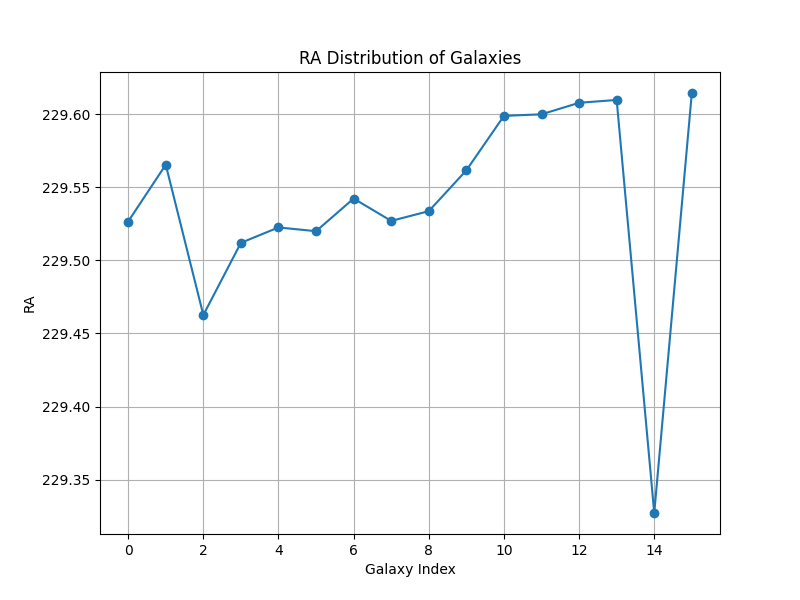
\includegraphics[width=0.8\textwidth]{Figure_2.png}
    \caption{Each data point on the plot represents a galaxy from the dataset. The position of each data point is determined by its RA coordinate (vertical axis) and its corresponding Galaxy Index value (horizontal axis).}
    \label{fig:figure2}
\end{figure}

% Results
\section{Results}
\input{Results}
% Bibliography
\begin{thebibliography}{9}
    % Add your bibliography items here
\end{thebibliography}

\end{document}
